O manipulador KUKA LBR iiwa é um braço robótico com 7 graus de liberdade projetado para trabalhar em conjunto com humanos no mesmo espaço de trabalho e de forma segura. De acordo com o fabricante, humanos e robôs podem trabalhar juntos em tarefas altamente sensíveis em estreita cooperação, o que abre a possibilidade de novas aplicações para a robótica \citep{KUKAmanual}. Isso é possível devido ao fato de que o robô apresenta sensores de torque em todos do eixos de rotação, e assim consegue se mover com precisão e detectar o contato com humanos e objetos. 

O propósito a que se destina o manipulador KUKA é declarado na sua nomenclatura. Enquanto que LBR se refere a palavra alemã ``\textit{Leichtbauroboter}'' cuja tradução literal é robô leve; o acrônimo iiwa vem do inglês ``\textit{intelligent industrial work assistant}'' equivalente a assistente de trabalho industrial inteligente, no português.

O robô em questão é classificado como um antropomorfo não compensado, visto que sua estrutura cinemática é da forma esférica-rotacional-esférica (SRS), similar ao braço humano (base, ombro, cotovelo e punho), como observa-se na FIG. \ref{fig:robo_iiwa}.

\begin{figure}[H]
    \centering
    \includegraphics[width=5cm]{Imagem/KUKA.jpg}
    \caption{Robô KUKA LBR iiwa}
    \label{fig:robo_iiwa}
    \begin{flushleft}
    Fonte: \citeauthor{KUKAapresentacao}, p. 22, 2017b.
    \end{flushleft}
\end{figure}

O KUKA LBR iiwa está disponível no mercado em duas versões, com capacidades de carga útil de 7 kg e 14 kg e apresentam alcance máximo de 800 mm e 820 mm, respectivamente. Na FIG. \ref{fig:dimensoes} é possível verificar o espaço de trabalho e os parâmetros das dimensões do robô, enquanto na TAB. \ref{tab:dimensoes} é informado seus valores para ambos os modelos. Mais informações podem ser encontrada no Apêndice \ref{apend:dim}.

\begin{figure}[h]
    \centering
    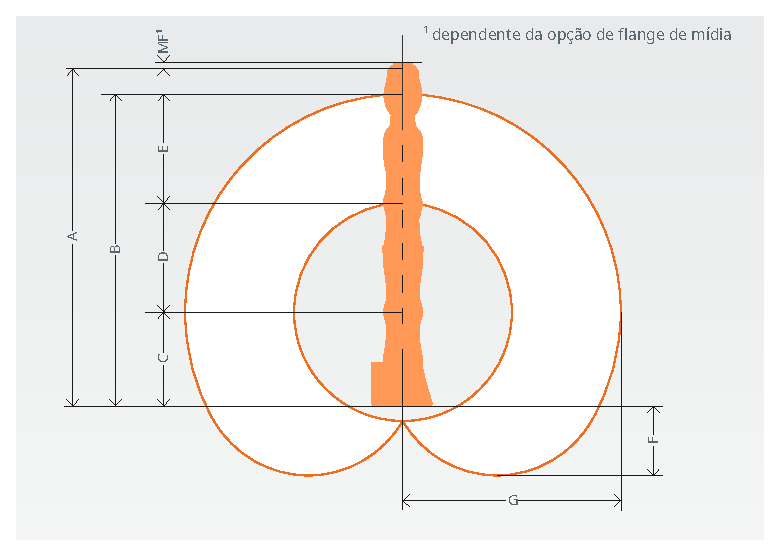
\includegraphics[width=0.48\textwidth]{Imagem/volume_trab.eps}
    \caption{Dimensões do KUKA LBR iiwa}
    \label{fig:dimensoes}
    \begin{flushleft}
    Fonte: KUKA, p. 30, 2017a. (Adaptação de     cores e tradução).
    \end{flushleft}
\end{figure}

\begin{table}[h]
    \centering
    \caption{Dimensões, em milímetros, dos parâmetros da FIG. \ref{fig:dimensoes}}
    \label{tab:dimensoes}
    \begin{tabular}{cccccccc}
    \toprule
        Robô & $A$ & $B$ & $C$ & $D$ & $E$ & $F$ & $G$ \\
    \midrule
         7 R800 & 1,266 & 1,140 & 340 & 400 & 400 & 260 & 800 \\
        14 R820 & 1,306 & 1,180 & 360 & 420 & 400 & 255 & 820 \\
    \bottomrule
    \end{tabular}
\end{table}

\subsection{Aplicações e Estudos de Casos}

Existem diversas áreas de aplicação em que o manipulador KUKA LBR é utilizado. Devido às suas características funcionais e sua adaptabilidade em trabalhar ao lado do fator humano, o robô é utilizado, principalmente, em indústrias de tecnologia e de produção em massa. As principais tarefas delegadas ao manipulador são aquelas de repetição monótona, como em funções de pintar, colar, aplicar, paletizar, embalar, medir e testar. Há também a utilização do robô na área de usinagem mecânica e montagem de peças.

% ANTES DA MODIFICAÇÃO Estudos de caso estão disponíveis no site da fabricante do robô, e vale ressaltar aqui, alguns em específico, como a solução desenvolvida pela KUKA para a montadora de veículos BMW, em uma de suas instalações localizada na cidade de Dingolfing na Alemanha.

Estudos de caso são apresentados na página web da fabricante do robô na qual algumas aplicações se destacam. Um exemplo é a solução desenvolvida pela fabricante KUKA para a montadora de veículos BMW em uma instalação localizada em Dingolfing, Alemanha. 

Em uma determinada etapa do processo de fabricação de veículos, os funcionários do Grupo BMW precisavam montar caixas de engrenagens de eixos dianteiros. Estes carregavam e levantavam peças de até 5 kg, de difícil acesso, com tolerâncias milimétricas de ajuste. A solução desenvolvida foi utilizar o robô KUKA LBR para montagem das engrenagens. O manipulador trabalha de forma suspensa e realiza o trabalho ``pesado'', poupando o esforço físico dos funcionários. 

%ANTES DA ALTERAÇÃO A garra foi projetada com revestimentos arredondados, protegendo os operadores de ferimentos. Além disso, sensores externos não são necessários, porque o LBR possui um sistema de sensor de torque articulado em cada um de seus sete eixos, fornecendo segurança aos operadores. (MUDEI PORQUE JÁ FALAMOS QUE TEM SENSOR DE TORQUE EM TODAS A JUNTAS, TENTEI AMENIZAR A REPETIÇÃO DA INFORMAÇÃO)

A garra foi projetada com revestimentos arredondados, protegendo assim os operadores de ferimentos. Além disso, sensores externos não são necessários devido à presença dos sensores de torque nas juntas que fornecem segurança aos operadores. Na FIG. \ref{fig:BMW} pode-se observar uma foto do robô operando na aplicação descrita. 

\begin{figure}[h]
    \centering
    \includegraphics[width=0.48\textwidth]{Imagem/BMW.jpg}
    \caption{Instalação de peças em superfícies complexas de um monobloco da BMW}
    \label{fig:BMW}
    \begin{flushleft}
    Fonte: \citeauthor{KUKAmanual}, p. 28, \citeyear{KUKAmanual}.
    \end{flushleft}
\end{figure}

Outro estudo de caso a ser mencionado é a utilização do manipulador pela fabricante de equipamentos eletrônicos Siemens. No âmbito da fabricação de estatores a Siemens, na unidade de Bad Neustadt, também na Alemanha, procurava por uma solução flexível para automatizar a atividade simples de entrega e posicionamento de peças, que até então era feita manualmente. 

A solução criada foi o desenvolvimento de uma célula flexível com o robô de construção leve KUKA LBR iiwa. Assim, o robô, assume a função de retirar a peça a ser processada --– o estator composto de um corpo básico de chapa elétrica e placa de alumínio --- do porta-peças e encaminhá-la a um torno que fará a sua usinagem. Após este processo, o robô apanha as peças, faz uma limpeza por sopro e as destina à estação de medição.

\begin{figure}[h]
    \centering
    \includegraphics[width=8cm]{Imagem/Siemens.jpg}
    \caption{Carregamento automático de um torno CNC na Siemens}
    \label{fig:SIEMENS}
    \begin{flushleft}
    Fonte: \citeauthor{KUKAmanual}, p. 21, \citeyear{KUKAmanual}.
    \end{flushleft}
\end{figure}

Outros estudos de caso aos quais a implementação do robô simplificou os processos tecnológicos, são de empresas como a Ford, Volkswagen e Perschmann Calibration GmbH. 

Nas indústrias da Ford, vários robôs foram instalados para aplicar um cordão de vedação em diversas peças. Eles sempre aplicam o material exatamente na mesma posição e na quantidade definida. Assim é possível obter uma boa vedação na carroceria e evitar um retrabalho na pintura, eliminando custos.

Já na montadora alemã, Volkswagen, o robô KUKA LBR iiwa participa de processos de montagem, colagem e soldagem. Trabalhando ao lado do fator humano, o robô realiza suas funções com precisão e eficiência, como é mostrado na FIG \ref{fig:VW}. 

\begin{figure}[h]
    \centering
    \includegraphics[width=8cm]{Imagem/VW.jpg}
    \caption{Montagem de peças na linha de produção}
    \label{fig:VW}
    \begin{flushleft}
    Fonte: \citeauthor{KUKAmanual}, p. 21, \citeyear{KUKAmanual}.
    \end{flushleft}
\end{figure}

A empresa  Perschmann Calibration GmbH, especialista em serviços de calibração, utiliza o manipulador como ferramenta de medição.  De acordo com o Dr. Detlef Rübesame, diretor Técnico da Perschmann Calibration, um cabelo humano tem aproximadamente \SI{50}{\micro\metre} de espessura, os fios de uma aranha, cerca de \SI{5}{\micro\metre}, e a precisão com a qual o robô faz sua calibração é de cerca de \SI{0,5}{\micro\metre}, um valor importante para manter a qualidade de seus serviços. Estes e outros estudos de caso endossam a importância do novo antropomorfo no mercado.
